\section{Theory}

Zeeman effect is the effect of splitting of a spectral line into several components in the presence of a static magnetic field. A shift in the energy level of one or both of the states involved in the transition results in a shift in the frequency/wavelength of the spectral line, which can be observed. Since the distance between the Zeeman sub-levels is a function of magnetic field strength, this effect is often used to measure magnetic field strength, for example that of  stars like the sun or plasma.

\subsection*{Normal Zeeman Effect}

The Zeeman effect that occurs for spectral lines resulting from a transition between
singlet states is traditionally called the normal effect.
For such states, the spin is zero and the total angular momentum $J$ is equal to the
orbital angular momentum $L$. When placed in an external magnetic field, the energy
of the atom changes because of the energy of its magnetic moment in the field. 

Mathematically, we can analyse this by considering a magnetic dipole. An external magnetic field will exert a torque on a magnetic dipole and the magnetic potential energy which results in

\begin{align}
    U(\theta) = -\mu \cdot B
\end{align}

where $\mu$ is the dipole moment. The magnetic dipole moment associated with the orbital angular momentum is given by,

\begin{align}
    \mu_\text{orbital} = \frac{e}{2m_e}L
\end{align}

where $L$ is the orbital angular momentum. By the quantization of angular momentum in the solution of the Schrodinger's equation, we know that the z-component of angular momentum is given by $L_z=m_l\hbar$, where $m_l$ is the magnetic quantum number. Then for a magnetic field in the z-direction, 

\begin{align}
    U = \frac{e}{2m_e}L_zB = m_l\frac{e\hbar}{2m_e}B
\end{align}

Hence, this gives equally spaced energy levels displaced from the zero field level by

\begin{align} \label{deltaE}
    \Delta E &= m_l\frac{e\hbar}{2m_e}B = m_l \mu_B B\\
    \text{where } \mu_B &= \frac{e\hbar}{2m_e} = 9.27 \times 10^{-24}\,\,J/T \nonumber
\end{align}

This displacement of the energy levels gives the uniformly spaced multiplet splitting of the spectral lines. 
Since there are $2l + 1$ values of $m_l$, each energy level
splits into $2l + 1$ levels. The selection rule
$\Delta m_l = \pm 1$ restricts the number of possible transition energies: $E_0 + e\hbar B/2m_e$, $E_0$,
and $E_0 + e\hbar B/2m_e$, corresponding to the transitions with $\Delta m_l = +1,\,0,\,-1$.

In this experiment, we observe the splitting of the Cd-spectral line at 643.8 nm into three lines, the so-called \textit{Lorentz triplets}. Cadmium has the electron structure, [Kr] $4d^{10}5s^2$, i.e.
the outer shell taking part in optical transitions is composed of the two $5s^2$
electrons representing a completed
electron shell. The transition seen here is $3^1d_2 \rightarrow 2^1p_1$.

\begin{figure}
    \centering
    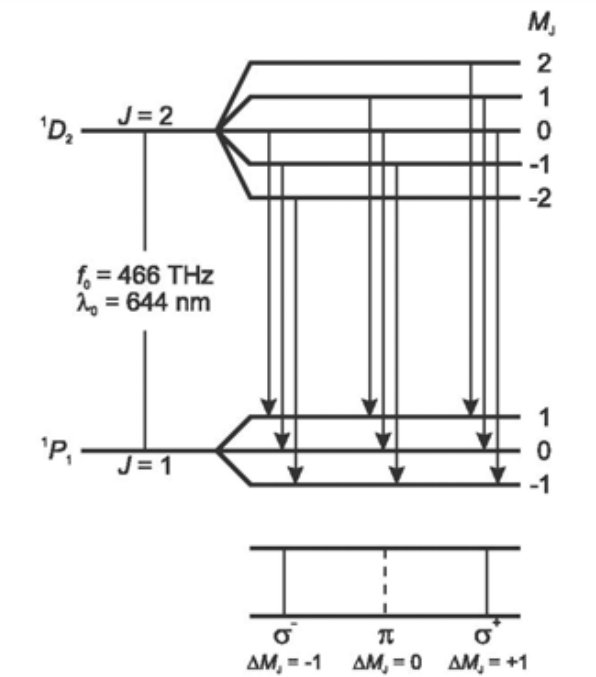
\includegraphics[width=.45\columnwidth]{images/th1.png}
    \caption{Level splitting and transitions of the normal Zeeman effect in Cadmium}
\end{figure}

When the magnetic field is in the transverse direction, $\Delta m_l = \pm 1$  transitions give $\sigma$-lines which are polarized vertically to the magnetic field. $\Delta m_l = 0$ transition gives a $\pi$-line in the middle, which is polarized parallel to the direction of the field.
However in a longitudinal field, we see only $\sigma$ lines which are right circular and left circular polarized ($\sigma^+$ and $\sigma^-$). 

% \begin{figure}
%     \centering
%     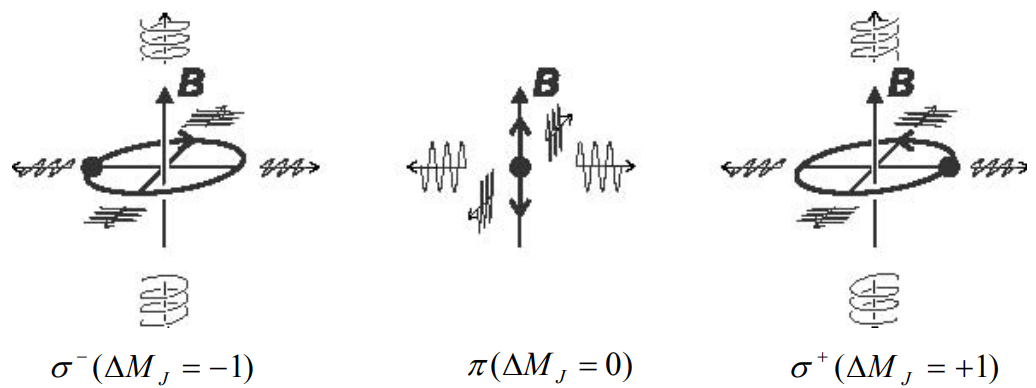
\includegraphics[width=.8\columnwidth]{images/th2.png}
%     \caption{Schematic representation of the polarization of the Zeeman components}
% \end{figure}

\begin{figure}
    \centering
    \begin{subfigure}[b]{0.48\textwidth}
        \centering
        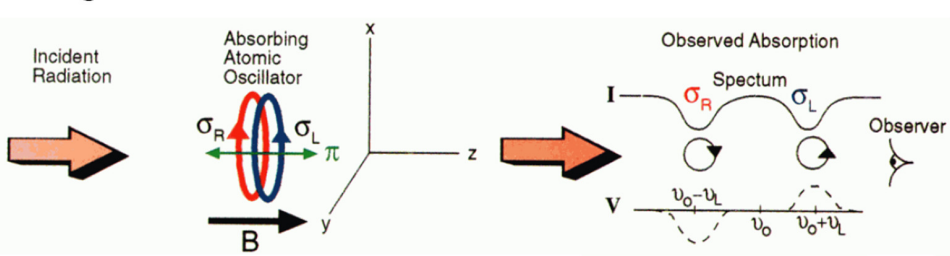
\includegraphics[width=\textwidth]{images/f1.png}
        \caption{Longitudinal Zeeman Effect}
    \end{subfigure}
    \begin{subfigure}[b]{0.48\textwidth}
        \centering
        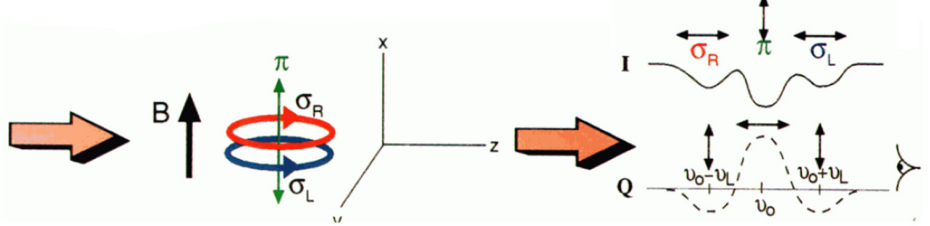
\includegraphics[width=\textwidth]{images/f2.png}
        \caption{Transverse Zeeman Effect}
    \end{subfigure}
    \caption{Schematic representation of the polarization of the Zeeman components}\label{fields}
\end{figure}

\subsection*{Anomalous Zeeman Effect}

The anomalous Zeeman effect appears on transitions where the net spin of the electrons is non-zero. Here the electron spins do not cancel each other and the
energy of an atomic state in a magnetic field depends on
both the magnetic moments of electron orbit and electron spin. In this experiment, we use the Cd $2^3s_1\rightarrow 2^3p_2$ transition at 508.58 nm to observe two groups of three $\sigma$
lines (in vertical polarization) and one group of three $\pi$ lines
in horizontal polarization.
% ==========================================================================
\section{Experimental Setup}

In this experiment, we use a Fabry-Perot interferometer to study the spectral lines. This instrument uses the phenomenon
of multiple beam interference that arises when light shines
through a cavity bounded by two reflective parallel surfaces. Each time the light encounters one of the surfaces,
a portion of it is transmitted out, and the remaining part
is reflected back. The net effect is to break a single beam into multiple beams which interfere with each other. If
the additional optical path length of the reflected beam
(due to multiple reflections) is an integral multiple of the
light's wavelength, then the reflected beams will interfere
constructively. More is the number of reflection inside the
cavity, sharper is the interference maximum. It makes use of multiple reflections which follow the interference condition for thin films. 

\begin{figure}
    \centering
    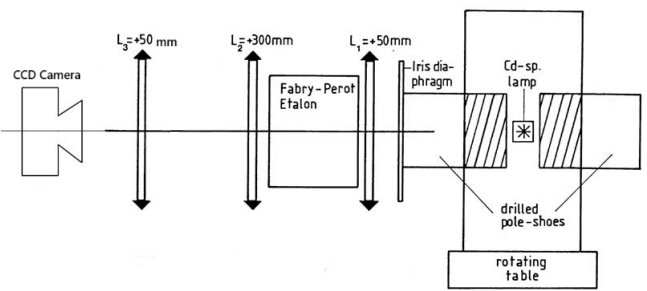
\includegraphics[width=1\columnwidth]{images/exp1.png}
    \caption{Schematic representation of the the optical components of the experimental setup}
\end{figure}

The net phase change is
zero for two adjacent rays, so the relation to find a maxima
is:

The difference in wave numbers of one of the $\sigma$ lines with respect to central $\pi$ line of the
same order is $\Delta k/2$. For this case,

\begin{align}
    \Delta E = hc\frac{\Delta k}{2}
\end{align}

Combining this with Eq. \ref{deltaE} with $\Delta m_l=1$, we get

\begin{align} \label{straight}
    \mu_B = hc\frac{\Delta k}{2B}
\end{align}

Now, $\Delta k$ can be calculated using,

\begin{align} \label{delk}
    \Delta k = \frac{1}{2\mu t}\left(\frac{\delta}{\Delta}\right)
\end{align}

The étalon consists of a quartz glass plate of $t=3$ mm thickness coated on both sides with a partially reflecting layer (90\% reflection, 10 \% transmission). Refractive index of quartz at 509 nm is $\mu=1.4519$ and
at 644 nm is $\mu=1.4560$. Here $\delta$ is mean of difference of squares of radii of different lines of same order of
interference and $\Delta$ is the mean of difference of squares of radii of different order, given by

\begin{align} \label{deltas}
    \delta_{n,xy} = R^2_{n,y}-R^2_{n,y}\text{ and }\Delta^x_n=R^2_{n+1,x}-R^2_{n,x}
\end{align}

Here, $n$ refers to the order of the ring and $x,\,y \in (a,b,c)$ where $a$ and $c$ are outer $\sigma$ lines and the middle $b$ is $\pi$ line. 

\subsection*{Apparatus}

\begin{enumerate}
    \item Cd-spectral lamp on rotating table, with drilled pole pieces
    \item A CCD camera
    \item A Fabry-Perot etalon
    \item Lenses (+50 mm and +300 mm)
    \item Polarizing filters
    \item Quarter-wave plate
    \item Software to analyse CCD output
    \item Optical Bench
\end{enumerate}